%\documentclass[compress]{beamer}
\documentclass[8pt]{beamer}

%-----------------------------------------------------------
% PACKAGES

%\usepackage[latin1]{inputenc}
\mode<presentation>

%\usepackage[T1]{fontenc}  
\usetheme{Warsaw}

\usepackage{graphicx}
%\usepackage[section]{placeins} % force � mettre l'image o� on veut
%\usepackage{float} %utiliser H pour forcer � mettre l'image o� on veut
\usepackage{lscape} %utilisation du mode paysage
%\usepackage{pslatex}
\usepackage{url}
%\usepackage{subfigure}
\usepackage{caption}
\usepackage{subcaption}

\usepackage{graphicx}
\usepackage{tabls}
\usepackage{afterpage}

%\usepackage[]{media9}
\usepackage{multimedia}

\usepackage{amsthm}
\usepackage{amssymb}
\usepackage{amsmath}
\usepackage{amsfonts}
\usepackage{amstext}
\usepackage{amsbsy}
\usepackage{mathbbol} 


\usepackage{epsfig}
%\usepackage{epsfig}
%\usepackage{cites}
\usepackage{epsf}
\usepackage{array}
\usepackage{color}

%-----------------------------------------------------------
% NEW  DEFINITIONS
%
%=================================================================================================
% new commands
% +++++++++++++++++++++++++++++++++++++++++++++++++++++++++++++++++++++++++++++++++++++++++++++++++
\newcommand{\nc}{\newcommand}

\renewcommand{\div}{\mbold{\nabla}\! \cdot \!}
\newcommand{\grad}{\mbold{\nabla}}
\newcommand{\divv}[1]{\boldsymbol{\nabla}^{#1}\! \cdot \!}
\newcommand{\gradd}[1]{\mbold{\nabla}^{#1}}
\newcommand{\mbold}[1]{\boldsymbol#1}
% latex shortcuts
\newcommand{\bea}{\begin{eqnarray}}
\newcommand{\eea}{\end{eqnarray}}
\newcommand{\be}{\begin{equation}}
\newcommand{\ee}{\end{equation}}
\newcommand{\bal}{\begin{align}}
\newcommand{\eali}{\end{align}}
\newcommand{\bi}{\begin{itemize}}
\newcommand{\ei}{\end{itemize}}
\newcommand{\ben}{\begin{enumerate}}
\newcommand{\een}{\end{enumerate}}
\usepackage{amsthm}
\newtheorem*{remark}{Remark}
% DGFEM commands
\newcommand{\jmp}[1]{[\![#1]\!]}                     % jump
\newcommand{\mvl}[1]{\{\!\!\{#1\}\!\!\}}             % mean value
\newcommand{\keff}{\ensuremath{k_{\textit{eff}}}\xspace}
% shortcut for domain notation
\newcommand{\D}{\mathcal{D}}
% vector shortcuts
\newcommand{\vo}{\mbold{\Omega}}
\newcommand{\vr}{\mbold{r}}
\newcommand{\vn}{\mbold{n}}
\newcommand{\vnk}{\mbold{\mathbf{n}}}
\newcommand{\vj}{\mbold{J}}
\newcommand{\eig}[1]{\| #1 \|_2}
%
\newcommand{\EI}{\mathcal{E}_h^i}
\newcommand{\ED}{\mathcal{E}_h^{\partial \D^d}}
\newcommand{\EN}{\mathcal{E}_h^{\partial \D^n}}
\newcommand{\ER}{\mathcal{E}_h^{\partial \D^r}}
\newcommand{\reg}{\textit{reg}}
%
\newcommand{\norm}{\textrm{norm}}
\renewcommand{\Re}{\textrm{Re}}
\newcommand{\Pe}{\textrm{P\'e}}
\renewcommand{\Pr}{\textrm{Pr}}
%
\newcommand{\resi}{R}
%\newcommand{\resinew}{\tilde{D}_e}
\newcommand{\resinew}{\widetilde{\resi}}
\newcommand{\resisource}{\widetilde{\resi}^{source}}
\newcommand{\matder}[1]{\frac{\textrm{D} #1}{\textrm{D} t}}
%
\newcommand{\Gammakj}{\Gamma_{k \to j}}

% extra space
\newcommand{\qq}{\quad\quad}
% common reference commands
\newcommand{\eqt}[1]{Eq.~(\ref{#1})}                     % equation
\newcommand{\eqts}[1]{Eqs.~(\ref{#1})}                     % equations
\newcommand{\fig}[1]{Fig.~\ref{#1}}                      % figure
\newcommand{\tbl}[1]{Table~\ref{#1}}                     % table
\newcommand{\sct}[1]{Section~\ref{#1}}                   % section
\newcommand{\app}[1]{Appendix~\ref{#1}}                   % appendix
\newcommand{\lem}[1]{Lemma~\ref{#1}}                   % lemma
\newcommand{\theo}[1]{Theorem~\ref{#1}}                   % theorem
%
\newcommand{\ie}{i.e.,\@\xspace}
\newcommand{\eg}{e.g.,\@\xspace}
\newcommand{\psc}[1]{{\sc {#1}}}
\newcommand{\rs}{\psc{R7}\xspace}
%
\newcommand\br{\mathbf{r}}
%\newcommand{\tf}{\varphi}
\newcommand{\tf}{b}
%
%\renewcommand{\dim}{\ensuremath{\texttt{dim}}\xspace}
%
\newcommand{\tcr}[1]{\textcolor{red}{#1}}
\newcommand{\tcb}[1]{\textcolor{blue}{#1}}
  \newcommand{\tcg}[1]{\textcolor{green}{#1}}
\newcommand{\mt}[1]{\marginpar{ {\tiny #1}}}

\newtheorem{theorem}{Theorem}[section]
\newtheorem{lemma}[theorem]{Lemma}

\newcommand{\bs}[1]{\mathbf{#1}}
\renewcommand{\bs}[1]{\vec{#1}}
%\newcommand{\dd}{\mathrm{d}}
\newcommand{\norm}{\textrm{norm}}
\renewcommand{\Re}{\textrm{Re}}
\newcommand{\Pe}{\textrm{P\'e}}
\renewcommand{\Pr}{\textrm{Pr}}

\newcommand{\resi}{R_e}
%\newcommand{\resinew}{\tilde{D}_e}
\newcommand{\resinew}{\widetilde{\resi}}
\newcommand{\matder}[1]{\frac{\textrm{D} #1}{\textrm{D} t}}

\newcommand{\divv}[1]{\vec{\nabla}^{#1}\! \cdot \!}
\newcommand{\gradd}[1]{\vec{\nabla}^{#1}}

\newcommand{\tcr}[1]{\textcolor{red}{#1}}
\newcommand{\tcb}[1]{\textcolor{blue}{#1}}
\newcommand{\tcm}[1]{\textcolor{magenta}{#1}}

%=================================================================================================

%============================================================
\date{\today}

%\addtobeamertemplate{footline}{\hfill\insertframenumber/\inserttotalframenumber\hspace{2em}\null}

\setbeamertemplate{footline}{
\leavevmode%
%\hbox{\hspace*{-0.06cm}
\begin{beamercolorbox}[wd=.5\paperwidth,ht=3.25ex,dp=1ex,center]{author in head/foot}%
	\usebeamerfont{author in head/foot}\insertshortauthor%~~(\insertshortinstitute)
\end{beamercolorbox}%
\begin{beamercolorbox}[wd=.25\paperwidth,ht=3.25ex,dp=1ex,center]{section in head/foot}%
	\usebeamerfont{section in head/foot} ANS Winter 2014 % \insertshorttitle
\end{beamercolorbox}%
\begin{beamercolorbox}[wd=.25\paperwidth,ht=3.25ex,dp=1ex,left]{section in head/foot}%
	\usebeamerfont{section in head/foot}\insertshortdate{}\hspace*{2em}
	\insertframenumber{} / \inserttotalframenumber %\hspace*{2ex}
\end{beamercolorbox}}%
%\vskip0pt%
%}

\beamertemplatetransparentcovered

\urldef{\ragusa}\url{jean.ragusa@tamu.edu}
\urldef{\delchini}\url{delcmo@tamu.edu}
\urldef{\berry}\url{ray.berry@inl.gov}
\urldef{\andrs}\url{David.Andrs@inl.gov}
\urldef{\martineau}\url{rcmartineau@gmail.com}

\title{APPLICATION OF THE REACTOR SYSTEM CODE RELAP-7 TO SINGLE- AND TWO-PHASE FLOW WATER-HAMMER PROBLEMS}

\author{Marc O. Delchini$^\star$, Jean C. Ragusa$^\star$, Ray Berry$^\ddagger$, David Andrs$^\ddagger$ and Richard Martineau$^\ddagger$}
\institute{
$^\star$   Texas A\&M University, College Station, TX, USA\\
$^\ddagger$ Idaho National Laboratory, Idaho Falls, ID, USA}
%
%%%%%%%%%%%%%%%%%%%%%%%%%%%%%%%%%%%%%%%%%%%%%%%%%%%%%%%%%%%%%%%%%%%%
\begin{document}
%%%%%%%%%%%%%%%%%%%%%%%%%%%%%%%%%%%%%%%%%%%%%%%%%%%%%%%%%%%%%%%%%%%%
%
\begin{frame}
\titlepage
\small{email:  {\delchini}, {\ragusa}, {\berry}, {\andrs}, {\martineau} }
\end{frame}
%
\begin{frame}
	\frametitle{Outline}
	\tableofcontents 
\end{frame}
%
%%%%%%%%%%%%%%%%%%%%%%%%%%%%%%%%%%%%%%%%%%%%%%%%%%%%%%%%%%%%%%%%%%%%%
\section{Background and Motivation}
%%%%%%%%%%%%%%%%%%%%%%%%%%%%%%%%%%%%%%%%%%%%%%%%%%%%%%%%%%%%%%%%%%%%%
\subsection{Relap-7: a Next-generation nuclear reactor safety code}
%%%%%%%%%%%%%%%%%%%%%%%%%%%%%%%%%%%%%%%%%%%%%%%%%%%%%%%%%%%%%%%%%%%%%
%
\begin{frame} 
\frametitle{The RELAP (Reactor Excursion and Leak Analysis Program) family of codes}

\begin{block}{Current industry standard: RELAP-5 (mod 3.2)}
\begin{itemize}
\item 6-equation two-phase flow model with time- and volume-averaged equations. The 6-eq model is ill-posed (non hyperbolic) and needs artificial viscosity and surface tension to be well-posed.
\item Semi-implicit in time with staggered spatial grids %(momentum grid half-shifted from the mass/energy grid)
\item Original model developed in the mid 1970s-early 1980s with continued enhancements since then.
\end{itemize}
\end{block}
%
\begin{block}{\tcm{Relap-7}: next-generation reactor safety code}
\begin{itemize}
\item \tcr{Goal}: To develop the next-generation reactor safety code by leveraging advances in numerical methods and computer hardware
\item \tcr{Means}: Use \tcm{MOOSE} (Multiphysics Object-Oriented Simulation Environment) to solve the multiphysics problem
\begin{itemize}
\item Fully implicitly in time (BDF-2 time integration)
\item Jacobian-free Newton Krylov for nonlinear solves
\item Leverage from existing libraries: Finite Element Method (\tcm{libmesh}), linear/nonlinear solve libraries (\tcm{PETSc, Hypre})
\end{itemize}
\end{itemize}
\end{block}
\end{frame}
%
%%%%%%%%%%%%%%%%%%%%%%%%%%%%%%%%%%%%%%%%%%%%%%%%%%%%%%%%%%%%%%%%%%%%
\subsection{Density-based (compressible) Solvers for Low-Mach Flow Problems}
%%%%%%%%%%%%%%%%%%%%%%%%%%%%%%%%%%%%%%%%%%%%%%%%%%%%%%%%%%%%%%%%%%%%%
%
\begin{frame}{All-speed compressible fluid flow solver}
\vspace{-5mm}
\begin{block}{Viscous regularization }
\textcolor{magenta}{Artificial viscosity} schemes based on the entropy production 
 (Guermond et al., {\it Entropy viscosity method for nonlinear  conservation laws}, JCP-2011)\\
\smallskip
%The \tcm{entropy viscosity method} is \tcr{discretization-independent} and was significantly tested in the supersonic regime (including using \tcr{continuous FEM}).
The \tcm{Entropy Viscosity Method (EVM)} : \\
\hspace{0.5cm} $\bullet$ is \tcr{discretization-independent}  \\
\hspace{0.5cm} $\bullet$ was tested in the supersonic regime only \\
%\hspace{0.5cm} $\bullet$ was used on unstructured meshes  \\
%\hspace{0.5cm} $\bullet$ achieved \tcr{high-order accuracy} for smooth solution
%and was significantly tested in the supersonic regime
%(including using \tcr{continuous FEM}) . 
\end{block}
\vspace{-3mm}
\begin{block}{All-speed fluid flow solver}
\begin{itemize}
\item low-Mach flow $\rightarrow$ incompressible limit.
\item numerical methods developed for supersonic flows may fail to solve low-mach flows.
\begin{itemize}
\item derive a fix and keep dissipative terms well-behaved thru low-Mach asymptotic studies
\end{itemize}
\end{itemize}
Low-Mach: huge disparity in speeds (pressure waves move much faster)
\begin{itemize}
\item Severely CFL-constrained if using explicit time-stepping
\item Best to use \tcr{implicit} time stepping
\begin{itemize}
\item Nonlinear system of equations%(preconditioner: pressure-correction ICE, for example)\\
\item Fits the JFNK formalism in MOOSE % where all physic components are tightly coupled \\
\end{itemize}
\end{itemize}
\end{block}
\end{frame}
%
%%%%%%%%%%%%%%%%%%%%%%%%%%%%%%%%%%%%%%%%%%%%%%%%%%%%%%%%%%%%%%%%%%%%%
\section{A Brief Review of the Entropy Viscosity Method for Conservation Laws}
%%%%%%%%%%%%%%%%%%%%%%%%%%%%%%%%%%%%%%%%%%%%%%%%%%%%%%%%%%%%%%%%%%%%%
\subsection{Basic Idea}
%%%%%%%%%%%%%%%%%%%%%%%%%%%%%%%%%%%%%%%%%%%%%%%%%%%%%%%%%%%%%%%%%%%%%
%
\begin{frame}{Quick overview of the entropy-based artificial viscosity formalism}

General scalar conservation law: $\boxed{\partial_t u + \div \vec{f}(u) = 0}$.

\begin{enumerate}
\item Determine an entropy pair ($s(u),\, \vec{\Psi}(u)$) for the PDE under consideration
\item Compute the entropy residual $\boxed{R_e:=\partial_t s(u_h) + \div \Psi(u_h)}$, in each cell $K$, at each quadrature point $x_q$
\item Compute the speed associated with this residual
\be
v_e^K(x_q) := h_K \frac{|R_e(x_q)|_K}{|s-\overline{s}|_\infty}
\ee
%The denominator is used to normalize the residual
%. It is the deviation of $E(u)$ from the domain average $\overline{E}$.
\item Define the kinematic viscosity (m$^2$/s) as
\be
\mu^K(x_q) := h_K \min \Big( \frac{1}{2} \max_{x\in K}|\vec{f}'(u(x))|, \, v_e^K(x_q) \Big)
\ee
\item Plug in the standard Galerkin weak form as a \tcm{viscous regularization} %(\tcm{it is really a straightforward technique})
\be
\int_V \big( \partial_t u_h + \div \vec{f}(u_h) \big) b \, dx + \tcm{\sum_K \int_K \mu_K \grad u_h \cdot  \grad b \, dx} = 0 \quad \forall b
\ee
\end{enumerate}
%
\end{frame}
%************************************************
\begin{frame}
\frametitle{Example: Burgers equation}
\begin{figure}
        \centering
        \begin{subfigure}[b]{0.37\textwidth}
                \centering
                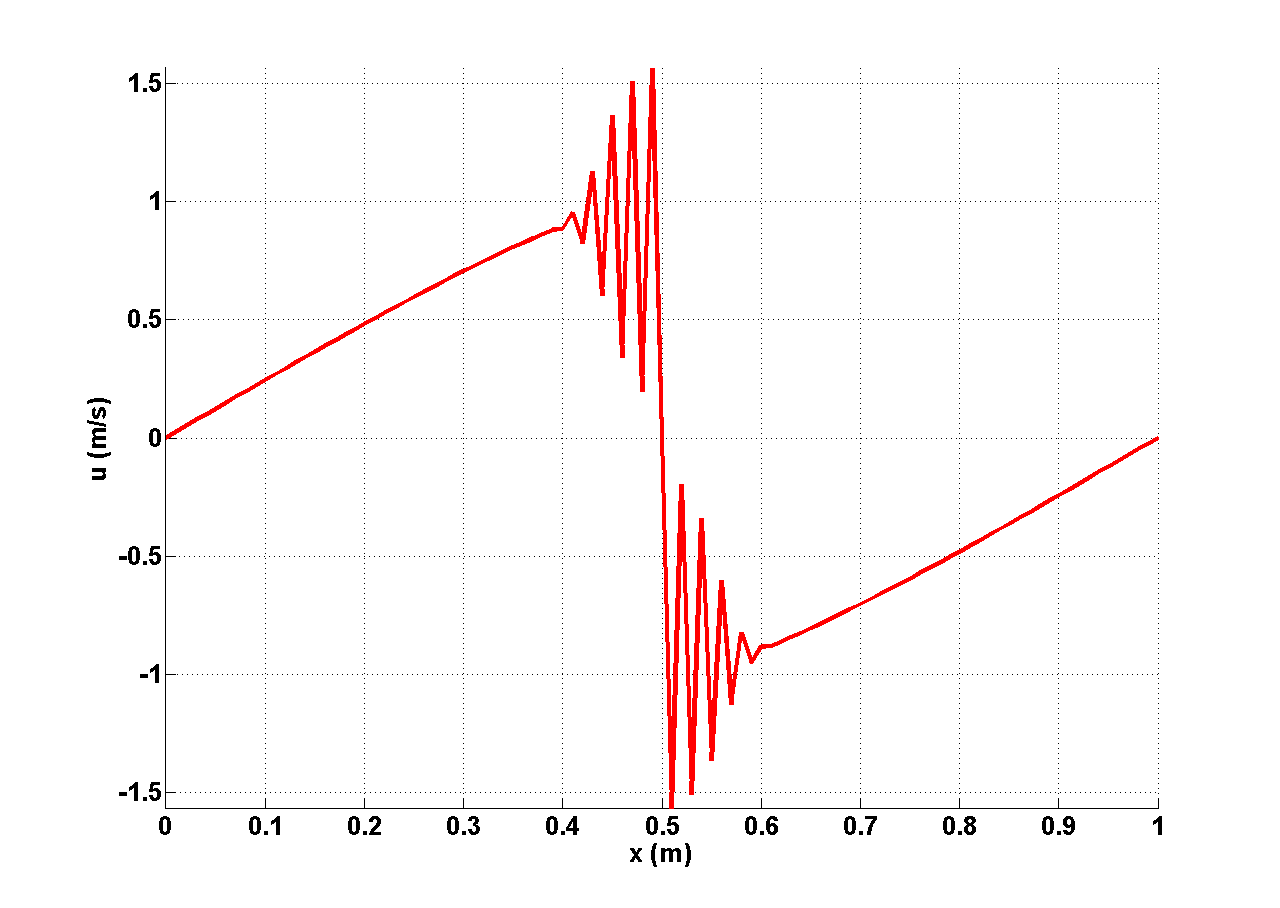
\includegraphics[width=\textwidth]{../../figures/presentation/1D_sol_free.png}
                \caption{Without stabilization.}
        \end{subfigure}%
        \begin{subfigure}[b]{0.37\textwidth}
                \centering
                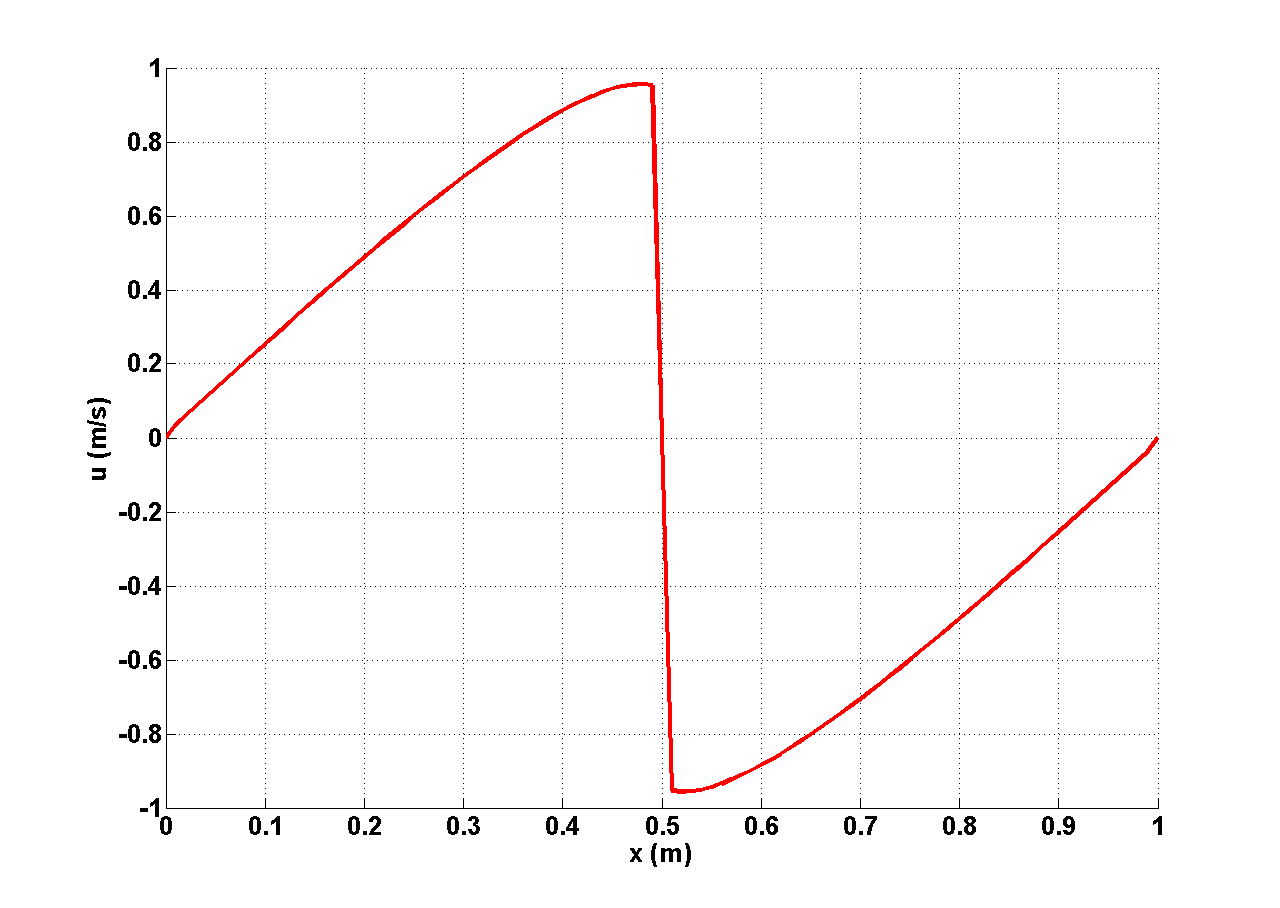
\includegraphics[width=\textwidth]{../../figures/presentation/1D_sol_fo.png}
                \caption{With first-order viscosity.}
        \end{subfigure}
        
        \begin{subfigure}[b]{0.37\textwidth}
                \centering
                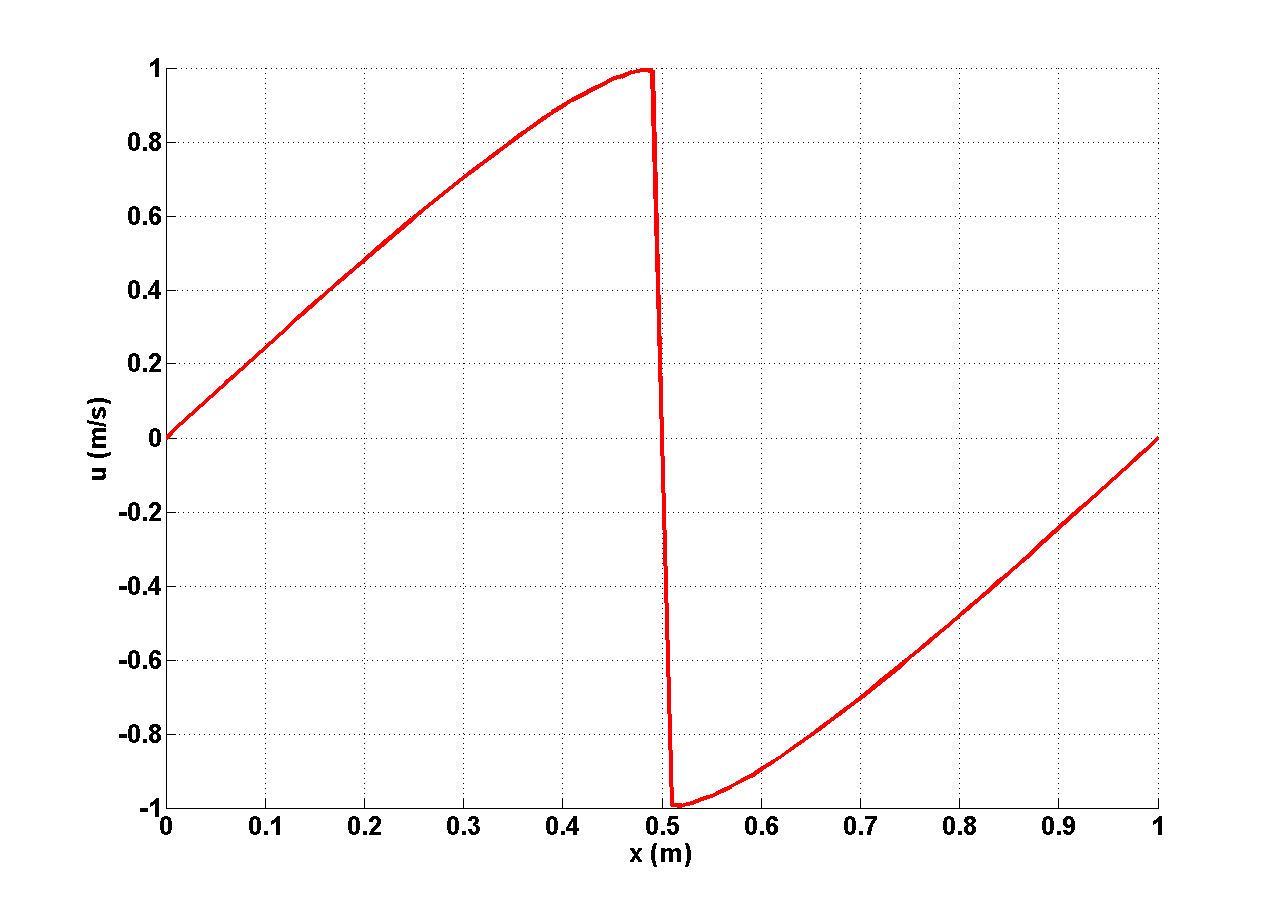
\includegraphics[width=\textwidth]{../../figures/presentation/1D_sol_ev.png}
                \caption{With the EVM.}
        \end{subfigure}
        \begin{subfigure}[b]{0.37\textwidth}
                \centering
                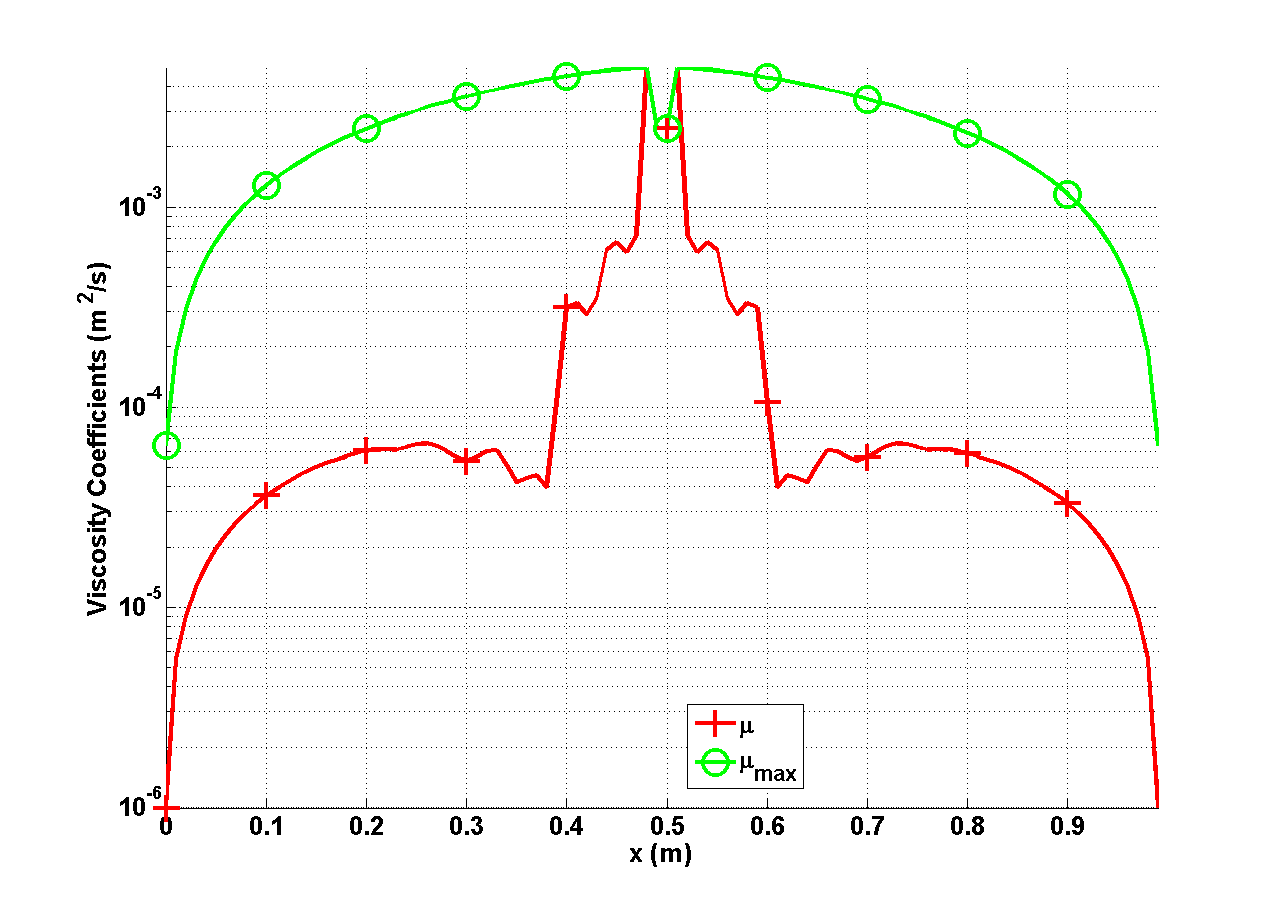
\includegraphics[width=\textwidth]{../../figures/presentation/1D_visc.png}
                \caption{Viscosity coefficient profiles.}
        \end{subfigure}
\end{figure}
\end{frame}
%
%%%%%%%%%%%%%%%%%%%%%%%%%%%%%%%%%%%%%%%%%%%%%%%%%%%%%%%%%%%%%%%%%%%%%
\subsection{Application to the Entropy Viscosity Method to the Euler Equations}
%%%%%%%%%%%%%%%%%%%%%%%%%%%%%%%%%%%%%%%%%%%%%%%%%%%%%%%%%%%%%%%%%%%%%
%
\begin{frame} 
\frametitle{Euler equations with viscous regularization}

The dissipative terms (in red) are added to the inviscid Euler equations.

\begin{block}{Euler equations with viscous regularization (final form)}
\begin{subequations}
\label{eq:euler_visc}
%
\begin{equation}
\partial_t \rho  + \div \left( \rho \vec{u} \right) = \textcolor{red}{\div \left( \kappa \grad \rho \right)} 
\end{equation}
%
\begin{equation}
\partial_t \left( \rho \vec{u} \right) + \div \left( \rho \vec{u} \otimes \vec{u} + P \mathbf{I} \right) = \textcolor{red}{\div \left( \mu \rho \grad^s \vec{u}  + \kappa \vec{u} \otimes \grad \rho \right) }
\end{equation}
%
\begin{equation}
\partial_t \left( \rho E \right) + \div \left[ \vec{u} \left( \rho E + P \right) \right] = \textcolor{red}{\div \left( \kappa \grad \left( \rho e \right) + \frac{1}{2}|| \vec{u} ||^2 \kappa \grad \rho +  \rho \mu \vec{u} \grad \vec{u}  \right) }
\end{equation}
\end{subequations}

\smallskip

where $\kappa$ and $\mu$ are positive viscosity coefficients.
\end{block}


\end{frame}
%**************************************************************************************************
%%************************************************
\begin{frame}{Supersonic formulation (Guermond, 2011)}
\vspace{-3mm}
\begin{block}{\textcolor{red}{Entropy-based viscosity coefficients} $\kappa_e$ and $\mu_e$ :}
\begin{itemize}
\item are based on the local entropy production,  
\item are numerically \tcm{evaluated} using the local entropy residual $\boxed{\resi(\vec{r},t) := \partial_t s + \vec{u} \cdot \grad s}$ %
%\begin{equation}
%\label{eq:ent_residual}
%\resi(\vec{r}, t) := \partial_t s + \vec{u} \cdot \grad s
%\end{equation}
\end{itemize}
%
\begin{equation}
\longrightarrow
\quad \mu^K_e(\vec{r}_q,t) =  h_K^2 \frac{  |\resi^K(\vec{r}_q,t) |}{|| s - \bar{s} ||_\infty}  
\qquad 
\kappa^K_e(\vec{r}_q,t) = \Pr \, \mu^K_e(\vec{r}_q,t)
\end{equation}
%
% $\Pr$ is a user-defined parameter and is usually taken in the range $[ 0.001; 1 ]$.
%\medskip

The denominator $|| s - \bar{s} ||_\infty$ is used for dimensionality purposes,
\textcolor{magenta}{no theoretical justification beyond a dimensionality argument}
\end{block}

\vspace{-1mm}
\begin{block}{First-order viscosities $\mu_{max}$ and $\kappa_{max}$}
\tcb{Upper bound} for the entropy viscosities (local Lax-Friedrichs) 
%
\begin{equation}
\label{eq:fo}
\mu^K_{\max}(\vec{r}_q, t) = \kappa^K_{\max}(\vec{r}_q, t) = \frac{h}{2}  \left( || \vec{u}(\vec{r}_q, t) || + c(\vec{r}, t) \right)
\end{equation}
If $\mu^K_{\max}$ and $\kappa^K_{\max}$ are used, the discretization scheme is over-dissipative and first-order.
\end{block}
%
\vspace{-3mm}
\begin{block}{Viscosity definitions}
\be
\mu^K = \min (\mu^K_e , \mu^K_{\max}) \qquad \kappa^K = \min( \kappa^K_e , \kappa^K_{\max})
\ee
\end{block}

\end{frame}
%
%%%%%%%%%%%%%%%%%%%%%%%%%%%%%%%%%%%%%%%%%%%%%%%%%%%%%%%%%%%%%%%%%%%%%
\section{Low Mach approach}
%%%%%%%%%%%%%%%%%%%%%%%%%%%%%%%%%%%%%%%%%%%%%%%%%%%%%%%%%%%%%%%%%%%%%
\subsection{New Formulation of the Entropy Residual}
%%%%%%%%%%%%%%%%%%%%%%%%%%%%%%%%%%%%%%%%%%%%%%%%%%%%%%%%%%%%%%%%%%%%%
%
\begin{frame} 
\frametitle{\textcolor{red}{Low-Mach issues} with current viscosity definitions}

Recall that 

\begin{equation}
\mu^K_e(\vec{r}_q,t) =  h_K^2 \frac{|\resi^K(\vec{r}_q,t) |}{\textcolor{magenta}{|| s - \bar{s} ||_\infty}} 
%\qquad
%\kappa^K_e(\vec{r}_q,t) = \Pr \, \mu^K_e(\vec{r}_q,t)
\end{equation}


\begin{block}{Issues with current formulation in the low-Mach limit}
\begin{itemize}
\item In the low-Mach Regime, the flow is known to be \textcolor{red}{isentropic}, resulting in very little entropy production
\item In practice, the entropy residual $\resi$ will be very small in that regime  (i.e., small numerator in the expression for the viscosity coefficients)
\item and so will be the denominator $|| s - \bar{s} ||_\infty$,
\item Thus, the formula for the viscosity coefficients are not determined \textcolor{red}{(ill-scaled) in the low-Mach limit}
\end{itemize}
\end{block}

\end{frame}
%**********************************************************************************************
\begin{frame}{Alternate definition of the entropy residual}

We can show that
\begin{equation}
\label{eq:ent_res}
\resi(\vec{r},t) := \partial_t s + \vec{u} \cdot \grad s = \matder{s} = \frac{s_e}{P_e} \underbrace{\left( \matder{P} - c^2 \matder{\rho} \right)}_{\resinew(\vec{r},t)} \nonumber 
\end{equation} 

\underline{Ideal for the demonstration:} 
$s$ is a function of $e$ and $\rho$, thus $\matder{s} = s_e\matder{e} + s_\rho \matder{\rho}$\\
\smallskip
Re-express the internal energy $e$ as a function of $P$ and $\rho$ through the EoS.

\begin{block}{Consequences}
\begin{itemize}
\item Residuals $\resi$ and $\resinew$ are proportional to one another\\
(for ideal gas law, $\frac{s_e}{P_e}= \frac{C_v}{P}$)
 %and will experience similar variations in space and time. 
\item We elect to employ $\resinew$ instead of $\resi$ %for the evaluation of the local entropy residual.
\item \tcr{{\it An analytical expression of the entropy function $s$ is no longer needed}} %: the residual $\resinew$ is evaluated using the local values of $P\,,\rho\,,u\,,c$ %pressure, density, velocity and speed of sound.
\item \textcolor{red}{Suitable normalizations for the residual} $\resinew$ can be devised (e.g., $P$, $\rho c^2$, $\rho c || \vec{u} ||$ or $\rho || \vec{u} ||^2$)
\end{itemize}
\end{block}
\end{frame}
%**********************************************************************************************
\begin{frame}{What is a proper normalization for $\resinew(\vec{r},t)$?}
\vspace{-3mm}
\begin{block}{Requirements} % {What is a proper normalization for $\resinew(\vec{r},t)$?}
\begin{enumerate}
\item To recover the incompressible results in the low-Mach limit (i.e., pressure fluctuations $\propto M^2$; divergence-free flow; incompressible continuity equation)
\item To remain valid and accurate for supersonic flows
\end{enumerate}
\end{block}
\vspace{-1mm}
We pose
\begin{equation}
\mu^K_e(\vec{r}_q,t)    = h_K^2 \frac{ | \resinew^K(\vec{r}_q,t) | }{\norm_P^\mu}    
%\end{equation} 
\quad
\text{and} 
\quad
%\begin{equation}
\kappa^K_e(\vec{r}_q,t) = h_K^2 \frac{ | \resinew^K(\vec{r}_q,t) | }{\norm_P^\kappa} 
\end{equation}

We now need to determine $\norm_P^\mu$ and $\norm_P^\kappa$. $\rightarrow$
\textcolor{red}{Asymptotic analysis} to determine the proper scaling in the low-Mach limit.

\vspace{-1mm}
\begin{block}{Non-dimensionalized variables}
\vspace{-3mm}
\begin{multline}
\label{eq:norm_param}
\rho^*   = \frac{\rho}{\rho_\infty}           ,\
u^*      = \frac{u}{u_\infty}                 ,\
P^*      = \frac{P}{\rho_\infty c^2_\infty}   ,\
E^*      = \frac{E}{c^2_\infty }              ,\\
x^* = \frac{x}{L_\infty}                      ,\
t^* = \frac{t}{L_\infty / u_\infty}           ,\ 
\mu^*    = \frac{\mu}{\mu_\infty}             ,\
\kappa^* = \frac{\kappa}{\kappa_\infty}       ,
\end{multline}
%
where  the subscript $\infty$ denote the far-field  quantities and the superscript $*$ stands for the non-dimensionalized variables. The reference Mach number is given by
%
\vspace{-2mm}
\begin{equation}
M_\infty = \frac{u_\infty}{c_\infty}
\end{equation}
\end{block}

\end{frame}
%********************************************************
\begin{frame} 
\frametitle{Scaled Euler equations with viscous regularization}

\begin{subequations} 
\label{eq:Euler_eq2}
%
\begin{equation}
\label{eq:euler_eq2_cont}
\partial_{t^*} \rho^*+ \divv{*}  \left(  \rho^* \vec{u}^*  \right) = \frac{1}{\tcr{\Pe_\infty}} \divv{*}  ( \kappa^* \gradd{*} \rho^* )
\end{equation}
%
\begin{multline}
\label{eq:euler_eq2_mom}
\partial_{t^*} \left( \rho^* \vec{u}^* \right) 
+ \divv{*} \left( \rho^* \vec{u}^*\otimes \vec{u}^* \right) 
+ \frac{1}{\tcb{M_\infty^2}}\gradd{*}  P^*  
= 
\frac{1}{\tcr{\Re_\infty}} \divv{*} \left( \rho^* \mu^* \gradd{s,*} \vec{u}^* \right)  \\
+
\frac{1}{\tcr{\Pe_\infty}} \divv{*} \left(\vec{u}^*\otimes \kappa^* \gradd{*}  \rho^* \right)
\end{multline}
%
\begin{multline}
\label{eq:euler_eq2_energy}
\partial_{t^*} \left( \rho^* E^* \right) 
+ \divv{*}  \left[ \vec{u}^* \left( \rho^* E^* + P^* \right) \right] 
=
\frac{1}{\tcr{\Pe_\infty}} \divv{*}  \left( \kappa^*  \gradd{*} (\rho^* e^*) \right)   \\
+
\frac{\tcr{M_\infty^2}}{\tcr{\Re_\infty}} \divv{*}  \left( \vec{u}^* \rho^* \mu^* \gradd{s,*} \vec{u}^* \right)
+ 
\frac{\tcr{M_\infty^2}}{2 \tcr{\Pe_\infty}} \divv{*}  \left(\kappa^* (u^*)^2 \gradd{*} \rho^* \right) \, ,
\end{multline}
%
\end{subequations}

\medskip

\textcolor{magenta}{with the non dimensional Reynolds $(\Re_\infty)$ and P\'eclet $(\Pe_\infty)$ numbers} :
%
\begin{equation}
\label{eq:ref_numb}
\boxed{\Re_\infty = \frac{u_\infty L_\infty}{\mu_\infty}} \quad \text{ and } \quad 
\boxed{\Pe_\infty = \frac{u_\infty L_\infty}{\kappa_\infty}} \, .
\end{equation}

\end{frame}
%%********************************************************
\begin{frame} 
\frametitle{\normalsize Low-Mach Asymptotics: How should $\Re$ and $\Pe$ scale with the Mach number?}

\begin{block}{Pressure spatial fluctuations}
To recover the low-Mach results that the leading order and first-order pressure terms ($P_0$ and $P_1$) are spatially constant, we require \textcolor{red}{$\Re_\infty = \Pe_\infty = 1$}. \\
$\longrightarrow$ pressure fluctuations $\propto M^2$
\end{block}

\begin{block}{Divergence of the flow}
With this scaling, one can also show that
\begin{equation}
\frac{1}{\gamma P_0} \frac{d P_0}{dt}=-\div \vec{u}_0
\quad \text{ and } \quad
\partial_t \rho_0 + \vec{u}_0 \cdot \div \rho_0 = 0 \, .
\end{equation}
$\longrightarrow$ steady-state divergence-free flows.
\end{block}

Therefore, by setting the $\Re_\infty=\Pe_\infty=1$, the \tcr{incompressible fluid results are retrieved in the low-Mach limit when employing the compressible Euler equations {\it with viscous regularization terms present}.}

\end{frame}
%%********************************************************
\begin{frame} 
\frametitle{Back to $\norm_P^\mu$ and $\norm_P^\kappa$}

From the definition of the entropy viscosity coefficient $\left( \kappa^K_e(\vec{r}_q,t)    = h_K^2 \frac{ | \resinew^K(\vec{r}_q,t) | }{\norm_P^\kappa} \right)$, we have
\begin{equation}
\label{eq:norm_relation}
\kappa_\infty 
= L_\infty^2  \frac{ \rho_\infty c_\infty^2 }{ L_\infty/u_\infty  \norm_{P,\infty}^{\kappa} }
\quad \to \quad \boxed{\norm_{P,\infty}^{\kappa} = \tcb{\Pe_\infty} \rho_\infty c_\infty^2} 
%= \frac{ \rho_\infty c_\infty^2 u_\infty L_\infty }{ \norm_{P,\infty}^{\kappa} } \, .
\end{equation}

Since $\tcb{\Pe}$ scales as \tcb{1},  we obtain:
%
\begin{equation}
\label{eq:norm_relation_bis}
\boxed{\norm_{P,\infty}^{\kappa} =  \rho_\infty c_\infty^2 } \, .
\end{equation}
%
\eqt{eq:norm_relation_bis} provides a proper normalization factor to define the $\kappa$ viscosity coefficient.\\

\medskip 
Similarly :  $\norm_{P,\infty}^{\mu} = \rho_\infty c_\infty^2 $.

\begin{block}{Thus, the new definitions for the viscosities in the low-Mach limit are}
\begin{equation}
\mu^K_e(\vec{r}_q,t)    = h_K^2 \frac{ | \resinew^K(\vec{r}_q,t) | }{ \rho_\infty c_\infty^2 }    \, ,
\quad
\text{and} 
\quad
\kappa^K_e(\vec{r}_q,t) = h_K^2 \frac{ | \resinew^K(\vec{r}_q,t) | }{ \rho_\infty c_\infty^2 } \, .
\end{equation}
\end{block}

\end{frame}
%********************************************************
\begin{frame}{Bridging the gap from low-Mach to supersonic}

\begin{block}{Answer from non-isentropic study with same methodology}
\begin{equation}
\mu^K_e(\vec{r}_q,t)    = h_K^2 \frac{ | \resinew^K(\vec{r}_q,t) | }{ \rho || \vec{u} ||^2 }    \, , \text{ and } 
\kappa^K_e(\vec{r}_q,t) = h_K^2 \frac{ | \resinew^K(\vec{r}_q,t) | }{ \rho c^2 } \, . \nonumber
\end{equation}
\end{block}

\begin{block}{Recall answer from low-Mach asymptotic study (previous slide)}
\begin{equation}
\mu^K_e(\vec{r}_q,t)    = h_K^2 \frac{ | \resinew^K(\vec{r}_q,t) | }{ \rho c^2 }    \, ,
\text{ and }  
\kappa^K_e(\vec{r}_q,t) = h_K^2 \frac{ | \resinew^K(\vec{r}_q,t) | }{ \rho c^2 } \, . \nonumber
\end{equation}
\end{block}

However, we want to keep the \textcolor{red}{all-speed aspect of the flow solver}, so

\begin{block}{New definitions}

\begin{subequations}
\begin{equation}
\mu^K_e(\vec{r},t)    = h_K^2 \frac{ | \resinew^K(\vec{r}_q,t) | }{\textcolor{magenta}{a(M) \rho \|\vec{u}\|^2 + (1-a(M)) \rho c^2}}  \, , \nonumber
\end{equation} 
\text{and} 
\begin{equation}
\kappa^K_e(\vec{r},t) = h_K^2 \frac{ | \resinew^K(\vec{r}_q,t) | }{ \rho c^2} \, . \nonumber
\end{equation}
\end{subequations}

\end{block}

\end{frame}
%%%%%%%%%%%%%%%%%%%%%%%%%%%%%%%%%%%%%%%%%%%%%%%%%%%%%%%%%%%%%%%%%%%%%
\subsection{1-D Numerical results using Relap-7}
%%%%%%%%%%%%%%%%%%%%%%%%%%%%%%%%%%%%%%%%%%%%%%%%%%%%%%%%%%%%%%%%%%%%%
\begin{frame}{1-D numerical results}
\begin{block}{Water-hammer test}
\begin{itemize}
\item Discretization of 1-D pipe: linear test function, BDF2, 500 cells.
\item Uniform pressure $P= 7 / MPa$, uniform velocity $u=-12.5 \ m/s$ and uniform temperature $T=517 \ K$.
\item Wall boundary conditions
\item Numerical solution showed at time $t=8.7 \times 10^{-4}, \ 6.8 \times 10^{-3}$ and $10^{-2}$ s.
\end{itemize}
\end{block}
\end{frame}
%************************************************
\begin{frame}{Single-phase water hammer}
\begin{figure}[H]
        \centering
        \begin{subfigure}[b]{0.5\textwidth}
                \centering
                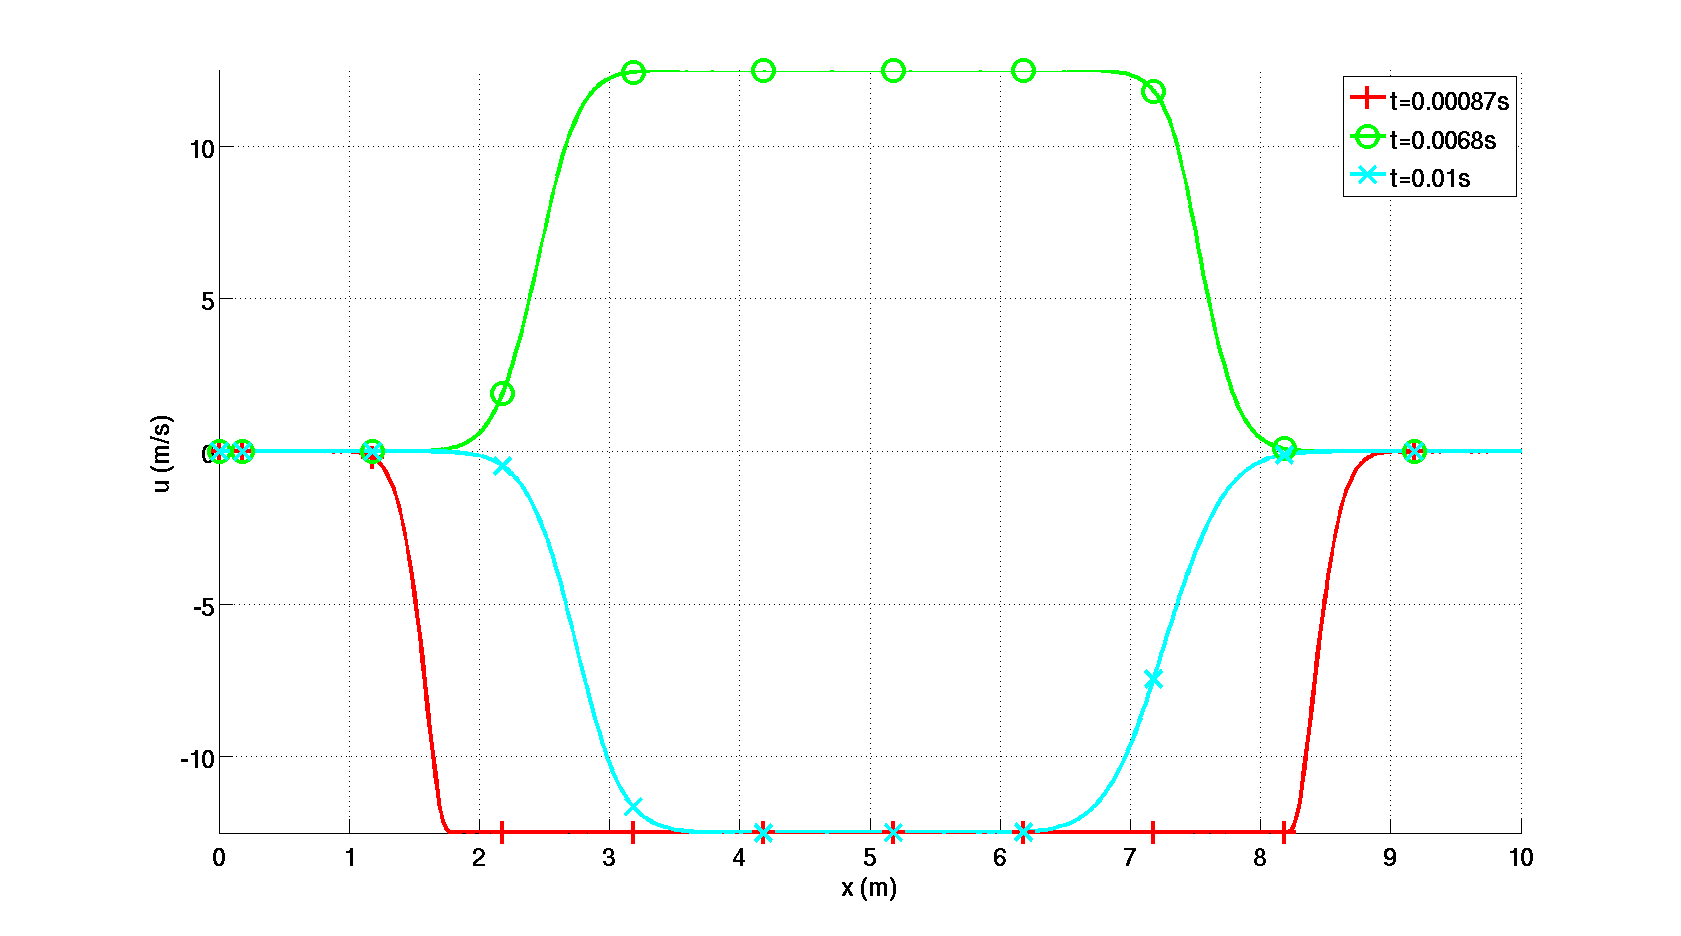
\includegraphics[width=\textwidth]{../../figures/paper/Plot_velocity_single_phase.png}
                \caption{Velocity}
                \label{fig:single-phase-vel}
        \end{subfigure}%
        \begin{subfigure}[b]{0.5\textwidth}
                \centering
                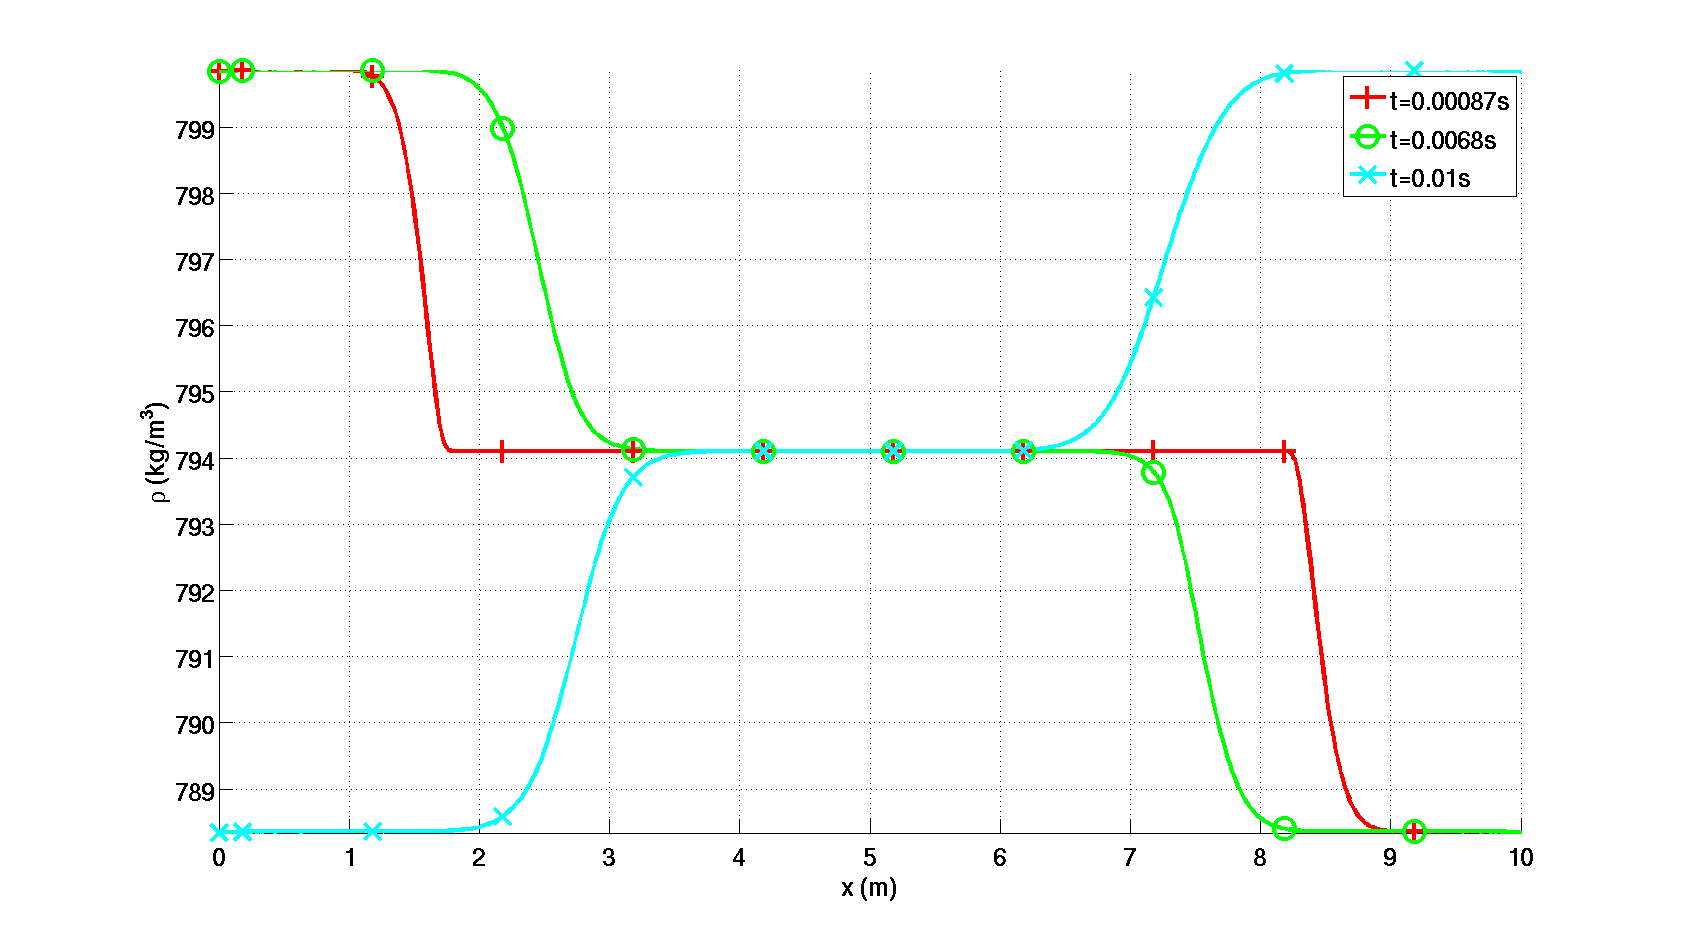
\includegraphics[width=\textwidth]{../../figures/paper/Plot_density_single_phase.png}
                \caption{Density}
                \label{fig:single-phase-density}
        \end{subfigure}
        
        \begin{subfigure}[b]{0.495\textwidth}
                \centering
                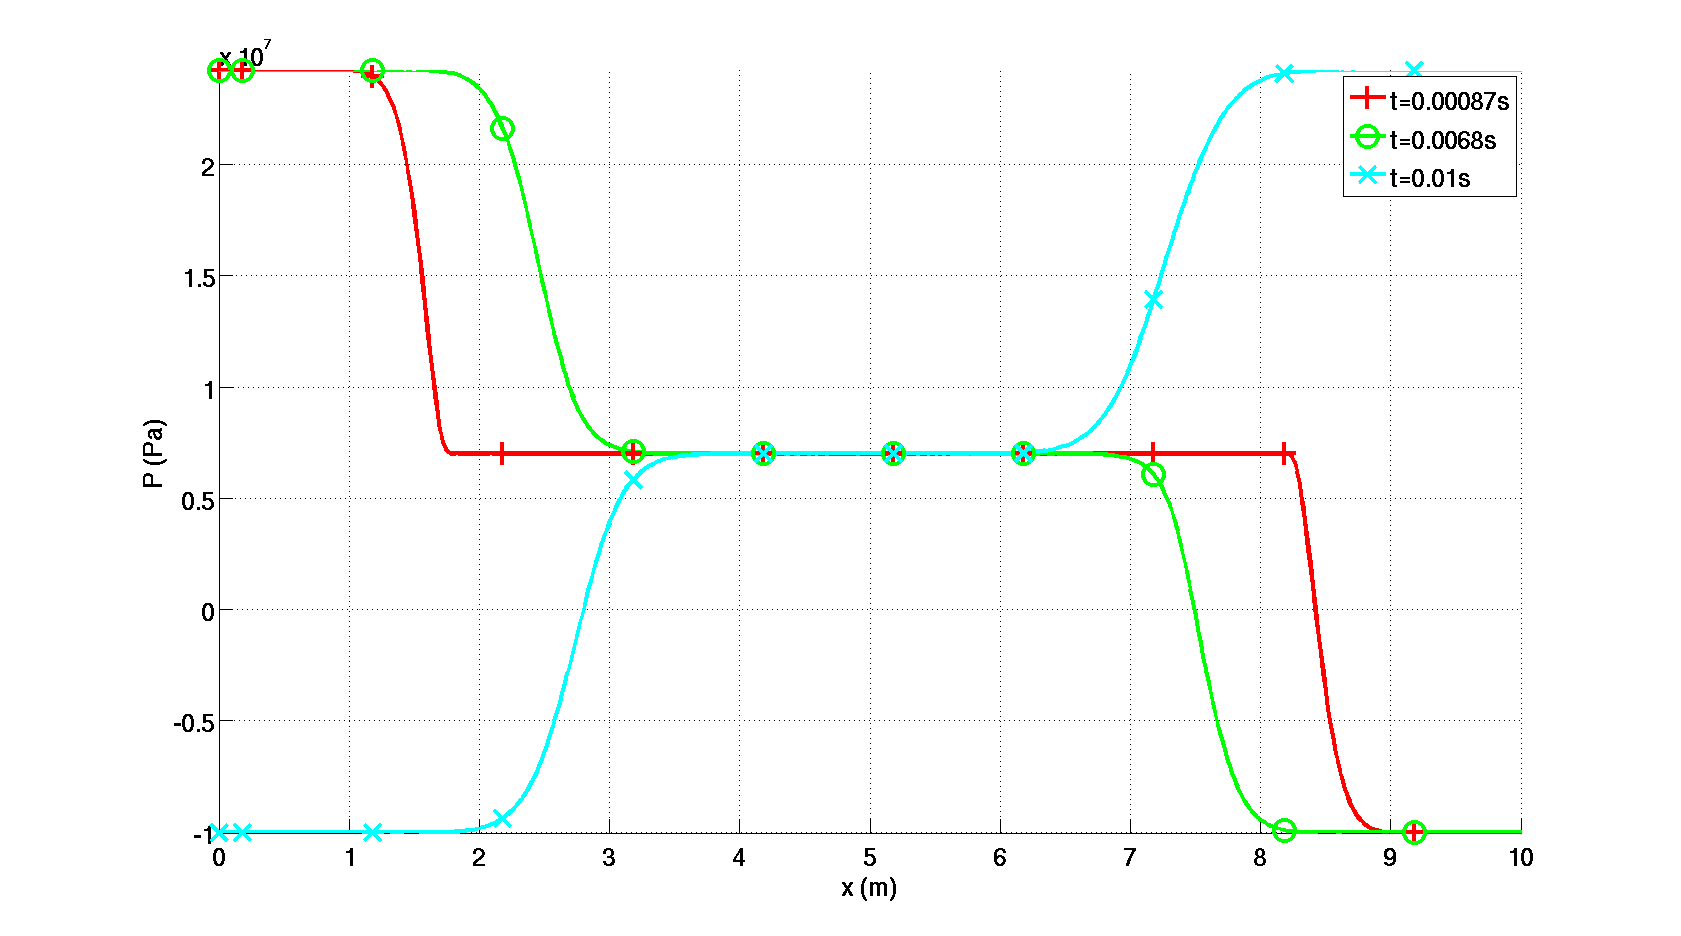
\includegraphics[width=\textwidth]{../../figures/paper/Plot_pressure_single_phase.png}
                \caption{Pressure}
                \label{fig:single-phase-press}
        \end{subfigure}        
        \begin{subfigure}[b]{0.495\textwidth}
                \centering
                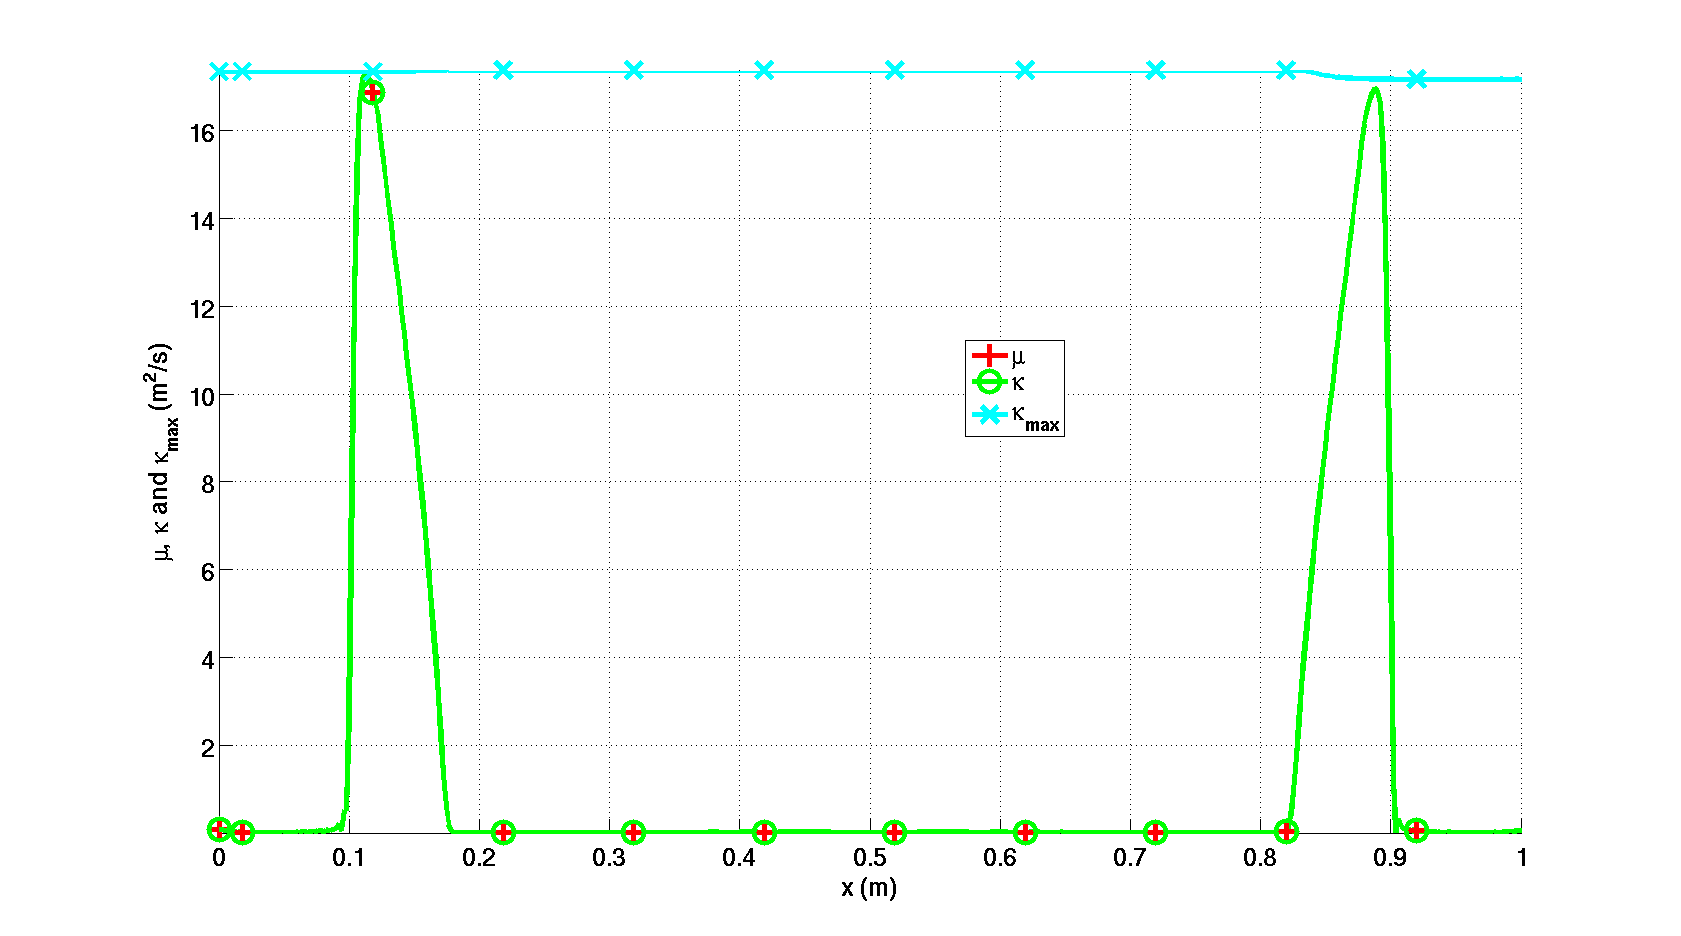
\includegraphics[width=\textwidth]{../../figures/paper/Plot_viscosity_single_phase.png}
                \caption{Viscosity coefficients}
                \label{fig:single-phase-visc}
        \end{subfigure}
        \caption{Numerical solutions of a water hammer at times $t=8.7 \times 10^{-4}, \, 6.8 \times 10^{-3} \text{ and } 10^{-3}$ s (the viscosity coefficients are only shown at time $t=8.7 \times 10^{-4}$ s).}\label{fig:single-phase}
\end{figure}
\end{frame}
%************************************************
%************************************************
\section{The seven-equation two-phase flow model}
%************************************************
%************************************************
\subsection{Description of the model}
%************************************************
%************************************************
\begin{frame}{The seven-equation model (SEM)}

\begin{block}{The model}
\begin{itemize}
\setlength{\itemsep}{10pt}
\item Each phase obeys the single-phase Euler equations: two continuity equations, two momentum equations and two energy equations
\item Seventh equation: volume fraction equation 
\item Exchange terms between phases: relaxation terms. These terms were derived using \emph{rational thermodynamic} and are consistent with the entropy minimum principle.
\item {\color{red}The system of equations is hyperbolic and has seven real waves}
\item The SEM degenerates to single-phase Euler equations when one phase disappears
\item The SEM degenerates into a 5-equation model when using infinite relaxation coefficients $\rightarrow$ Chapman-Enskog expansion.

\item \tcr{Numerical methods applied to the SEM : discontinuous schemes so far }
\end{itemize}
\end{block}

\end{frame}
%************************************************
%************************************************
\subsection{The entropy viscosity method applied to the Seven-Equation model}
%************************************************
%************************************************
\begin{frame}{Viscous regularization for the SEM (written here with variable area $A$)}

\begin{block}{}
\begin{subequations}
\begin{equation}
\partial_t \left( \alpha_k  A\right) + \vec{u}_{int} A \cdot \grad \alpha_k = {\color{red}A \mu_P \left( P_k - P_j \right)} + {\color{blue}\div \vec{l}_k}  
\end{equation}
%
\vspace{-2mm}
%
\begin{equation}
\partial_t \left( \alpha_k \rho_k A \right) + \div \left( \alpha_k \rho_k \vec{u}_k A \right) = {\color{blue}\div \vec{f}_k} 
\end{equation}
%
\vspace{-4mm}
%
\begin{multline}
\partial_t \left( \alpha_k \rho_k \vec{u}_k A \right) + \div \left[ \alpha_k A \left( \rho_k \vec{u}_k\otimes \vec{u}_k + P_k\mathbb{I}\right) \right] =   \\
\alpha_k P_k \grad A +  P_{int} A \grad \alpha_k +  {\color{red}A \lambda_u \left( \vec{u}_j - \vec{u}_k \right)} +{\color{blue}\div \mathbb{g}_k}
\end{multline}
%
\vspace{-4mm}
%
\begin{multline}
\partial_t \left( \alpha_k \rho_k E_k A \right) + \div \left[ \alpha_k A \vec{u}_j \left( \rho_k E_k + P_k \right) \right] =  \\
P_{int} \vec{u}_{int} A \grad \alpha_k - {\color{red}\mu_P \bar{P}_{int} \left( P_k-P_j \right)} +{\color{red}\bar{\vec{u}}_{int} A \lambda_u \left( \vec{u}_j - \vec{u}_k \right)} + {\color{blue}\div \vec{h}_k} 
\end{multline}
\end{subequations}
\end{block}
%
\vspace{-2mm}
%
\begin{block}{Viscous regularization: \tcm{same procedure} as with single-phase Euler equations}
\begin{equation}
\left\{
\begin{array}{lcl}
{\color{blue}\vec{l}_k} = A \beta_k \grad \alpha_k \\ 
{\color{blue}\vec{f}_k} = \alpha_k A {\color{magenta}\kappa_k}  \grad \rho_k + \rho_k \vec{l}_k& & \\
{\color{blue}\mathbb{g}_k} = \alpha_k A \rho_k {\color{magenta}\mu_k} \grad^s \vec{u}_k + \vec{u}_k \otimes \vec{f}_k & & \\
{\color{blue}\vec{h}_k} = \alpha_k A {\color{magenta}\kappa_k} \grad(\rho_k e_k) - \frac{||\vec{u}_k||^2}{2} \vec{f}_k + \vec{u} \cdot \mathbb{g}_k + \rho_k e_k \vec{l}_k & &
\end{array}
\right.
\nonumber
\end{equation}
Note: the viscous flux ${\color{blue}\vec{l}_k}$ plays no part in the entropy minimum principle; we used analogy with Burgers to determine it.
\end{block}
\end{frame}
%************************************************
\begin{frame}{An all-Mach flow definition of the viscosity coefficients}
Same definition as for Euler equations:
\begin{block}{\normalsize $\mu_k(\vec{r},t)    = \min \Big (\mu_{k,\max}(\vec{r},t), \mu_{k,e} (\vec{r},t)    \Big)$, and $\kappa_k(\vec{r},t) = \min \Big (\mu_{k,\max}(\vec{r},t), \kappa_{k,e} (\vec{r},t) \Big )$} 
\hspace{0.5cm} $\bullet$ $\ \kappa_{k,\max}(\vec{r},t)  = \mu_{k,\max} (\vec{r},t) = \frac{h}{2} \Big ( ||\vec{u}_k|| + c_k \Big )$.  \\ [3pt]
%
\hspace{0.5cm} $\bullet$ $\kappa_{k,e}(\vec{r},t) = \frac{h^2 \max(\resinew_k, J_k)}{ \textcolor{blue}{\rho_k c_k^2} }$ and
$\mu_{k,e}(\vec{r},t)    = \frac{h^2 \max(\resinew_k, J_k)}{ \textcolor{red}{\norm_{k,P}^\mu}}$  \\ [3pt]
%
\hspace{0.5cm} $\bullet$ $\resinew_k= \frac{DP_k}{Dt} - c_k^2 \frac{D\rho_k}{Dt}$ and $J_k = ||\vec{u_k} || \max \left( [[\ \grad P_k \cdot \vec{n}\ ]]  ,\ [[c_k^2 \grad \rho_k \cdot \vec{n} \ ]]\right)$ \\[3pt]
%
\hspace{0.5cm} $\bullet$ $\textcolor{red}{\norm_{k,P}^\mu} = a_k(M_k) \rho_k || \vec{u}_k ||^2 + (1-a_k(M_k)) \rho_k c_k^2$ \\ [4pt]
%
\hspace{0.5cm} $\bullet$ $\lim_{M_k \to 0} a_k(M_k) = 0$ and $\lim_{M_k \to + \infty} a_k(M_k) = 1$
\end{block}
%
Same definition as for Burger's equation:
\begin{block}{\normalsize $\beta_k(\vec{r},t) = \min \Big (\beta_{k,\max}(\vec{r},t), \beta_{k,e} (\vec{r},t) \Big )$}
\hspace{0.5cm} $\bullet$ $\beta_{max} = \frac{h}{2} || \vec{u}_{int} ||$ 
%and $\beta_{k,e} = h^2 \frac{\max( R_{k,\alpha}, J_{k,\alpha} )}{|| \eta_k - \bar{\eta}_k ||_\infty}$  \\ [3pt]
and $\beta_{k,e} = h^2 \frac{ R_{k,\alpha}}{|| \eta_k - \bar{\eta}_k ||_\infty}$  \\ [3pt]
\hspace{0.5cm} $\bullet$ $R_{k,\alpha} = \partial_t \eta_k + \vec{u}_{int}\cdot \grad \eta_k$ with $\eta_k = \frac{\alpha_k^2}{2}$ %and $J_{k,\alpha} = ||\vec{u}_{int} || \  [[\ \grad \alpha_k \cdot \vec{n}\ ]]$
\end{block}
\end{frame}
%**************************************************************
%**************************************************************
\subsection{1-D numerical results using Relap-7}
%**************************************************************
%**************************************************************
\begin{frame}{Two-phase flow 1-D water hammer}
\begin{center}
\movie[width=6cm,height=4cm,showcontrols=true,externalviewer]{\includegraphics[width=6cm,height=4cm]{engr.pdf}}{../../movies/water-hammer-test-pressure.avi}
\end{center}
\end{frame}
%************************************************
\begin{frame}{1-D hydrostatic test}
\begin{center}
\movie[width=6cm,height=4cm,showcontrols=true,externalviewer]{\includegraphics[width=6cm,height=4cm]{engr.pdf}}{../../movies/hydrostatic-test-200-cells-Aintmax-1e2-coeff-1em2.avi}
\end{center}
\end{frame}
%************************************************
\section{Conclusions}
\begin{frame}{Conclusions and future work}
\begin{block}{Euler equations}
\begin{itemize}
\item removed the need to have an entropy function
\item extended the EVM to low-Mach flows through a low-Mach asymptotic analysis 
\item validated our approach with $1$-D water-hammer test.
\end{itemize}
\end{block}
\begin{block}{The seven-equation two-phase flow model (SEM)}
\begin{itemize}
\item derived a viscous regularization for the SEM
\item defined the viscosity coefficients using the same methodology as for single-phase flow equation
\item our approach was validated by $1$-D results: water-hammer and hydrostatic tests.
\end{itemize}
\end{block}
\begin{block}{MOOSE/RELAP-7}
Fully  implicit temporal discretization with {\it continuous} FEM through MOOSE\\
Used in the next-gen nuclear reactor safety code RELAP-7
\end{block}
\end{frame}
%************************************************
\begin{frame}
\begin{center}
Thank you for your attention. \\
\bigskip
Questions / Comments ?
\end{center}
\end{frame}
%************************************************
\end{document}